\begin{frame}[fragile]{Indentation}
    \tit{Python Indentation}
    Indentation is a very important concept of Python because without proper indenting the Python code, 
    you will end up seeing IndentationError and the code will not get compiled.



    In simple terms indentation refers to adding white space before a statement.
    \pause
    \begin{lstlisting}[numbers=left,showstringspaces=false,language=python]
        Username = 'Omar_213'  
        if Username == 'Omar_213': 
            print('Logging on to website...')
            password=input('Enter your password') 
        else: 
            print('You are in the wrong place.') 
        print('All set !')
        \end{lstlisting}        
\end{frame}
\begin{frame}[fragile]{Indentation}
    \tit{Python Indentation Rules}
Python uses 4 spaces as default indentation spaces. However, the number of spaces can be anything, it is up to the user. 
But a minimum of one space is needed to indent a statement.
\begin{itemize}
    \item The first line of python code cannot have Indentation.
    \item Indentation is mandatory in python to define the blocks of statements.
    \item The number of spaces must be uniform in a block of code.
    \item It is preferred to use whitespaces instead of tabs to indent in python. Also, either use whitespace or tabs to indent, intermixing of tabs and whitespaces in indentation can cause wrong indentation errors.
\end{itemize}
\end{frame}
\begin{frame}[fragile]{Indentation}
\tit{Benefits of Indentation in Python}
\begin{itemize}
    \item Indentation of code leads to better readability, although the primary reason for indentation in python is to identify block structures.
    \item Missing \verb|{| and \verb|}| errors that sometimes popup in \verb|c,c++| languages (or other languages) can be avoided in python, also the number of lines of code is reduced.
\end{itemize}
\end{frame}
%TODO: if...else 
    %*Syntax
    %*Example
    %*Common Errors
\begin{frame}[fragile]{Conditions}
    \tit{\texttt{if} statement}
    Some programming problems need special treatment. 
    
    
    Let consider the following situation:
\begin{block}{}
Write a program that asks the user's age, then prints out the message "You are still young!" if his age is less than 30.
\end{block}
\pause 
to solve this problem, we need to use \texttt{if} statement given by the following syntax:
\begin{lstlisting}[numbers=left,showstringspaces=false,language=python] 
    if (test): #condition
        block of instructions #body
\end{lstlisting}
    \pause
\begin{itemize}[<+->]
    \item An \verb|if| statement executes the statements if the condition is true, and ignores it if the condition is false.
    \item The block of instructions must starts with and indentation and will end at the first unindented statement. 
\end{itemize}
\end{frame}
\begin{frame}[fragile]{Conditions}
    \begin{figure}
        \begin{center}
            \resizebox{.3\linewidth}{!}{
    
    \tikzstyle{decision} = [diamond, aspect=2, align=center, draw, fill=green!20, 
        text width=5.5em, text badly centered, node distance=2.5cm, inner sep=0pt]
    \tikzstyle{block} = [rectangle, aspect=2, align=center, draw, fill=blue!20, 
        text width=5em, text centered, rounded corners, minimum height=3em]
    \tikzstyle{line} = [draw, -latex']
    \tikzstyle{cloud} = [draw, ellipse,fill=red!20]
        
    \begin{tikzpicture}[node distance = 1.5cm, auto]
        % Place nodes
        \node [cloud] (init) {begin if};
        \node [decision,below of=init] (test) {test (condition)};
        \node [block, below of=test, node distance=2.5cm] (body) {body};
        \node [cloud, below of=body] (end) {end if};
        % Draw edges
        \path [line,dashed] (init) -- (test);
        \draw [line]  (test) --node[right] {True}  (body);
        \draw [line]  (test.west) |- (-2,-2.5) node[left] {False} |- (end.west);
        \path [line] (body) -- (end);
    \end{tikzpicture}}
    \end{center}
    \caption{Python \texttt{if} Statement Flowchart}
    \end{figure}
    \pause

    Therefore, the solution of the previous situation is:
\begin{lstlisting}[numbers=left,showstringspaces=false,language=python]
age=int(input("How old are you")) 
if (age<30):
    print("You are still young!")
\end{lstlisting}

\end{frame}
\begin{frame}[fragile]{Conditions}
\tit{\texttt{if...else} statements}
\begin{minipage}{.49\textwidth}
 \begin{block}{}
        If we have two outputs based on whether
        the condition is true or false,  we use the \fbox{\texttt{if...else}} statements
        \pause 
        \begin{itemize}[<+->]
            \item When the condition evaluates to \texttt{True}  executes the \fbox{\texttt{body\_of\_if}} and the \fbox{\texttt{body\_of\_else}} is skipped.
            \item When the condition evaluates to \texttt{False}
        the \fbox{\texttt{body\_of\_if}} is skipped and the \fbox{\texttt{body\_of\_else}} executes.
        \end{itemize}
 \end{block}
\end{minipage}
\begin{minipage}{.5 \textwidth}
    \begin{figure}
        \begin{center}
            \resizebox{.6\linewidth}{!}{
    \tikzstyle{decision} = [diamond, aspect=2, align=center, draw, fill=green!20, 
        text width=5.5em, text badly centered, node distance=2.5cm, inner sep=0pt]
    \tikzstyle{block} = [rectangle, aspect=2, align=center, draw, fill=blue!20, 
        text width=5em, text centered, rounded corners, minimum height=3em]
    \tikzstyle{line} = [draw, -latex']
    \tikzstyle{cloud} = [draw, ellipse,fill=red!20]    
    \begin{tikzpicture}[node distance = 1.5cm, auto]
        % Place nodes
        \node [cloud] (init) {begin if};
        \node [decision,below of=init] (test) {test (condition)};
        \node [block, below of=test, node distance=2.5cm] (body1) {body if};
        \node [block, below of=body1, node distance=2.5cm] (body2) {body else};
        \node [cloud, below of=body2] (end) {end if};
        % Draw edges
        \path [line,dashed] (init) -- (test);
        \draw [line]  (test) -- (body1);
        \draw [line]  (test.west) |- (-2,-2.5) node[left] {False} |- (body2.west);
        \path [line] (body1.east) |-(2,-5)|- (end.east);
        \path [line] (body2) -- (end);
    \end{tikzpicture}}
    \end{center}
    \caption{\texttt{if..else} Flowchart}
    \end{figure}
\end{minipage}
\end{frame}
\begin{frame}[fragile]{Conditions}
The syntax of \texttt{if...else} statement is:
\begin{lstlisting}[numbers=left,showstringspaces=false,language=python]
if conditional_test:
    body_of_if
else:
    body_of_else
\end{lstlisting}
\pause
\begin{example}
Write a program that asks the user to enter two numbers, then prints out the max between them without using any built-in function or module.
\end{example}
\pause
\begin{lstlisting}[numbers=left,showstringspaces=false,language=python]
a,b=int(input("Give the first number")),int(input("Give the second number"))
if (a>=b):
    print(a)
else:
    print(b)
\end{lstlisting}
\end{frame}
\begin{frame}[fragile]{Conditions}
\begin{example}
    Let suppose that we want to develop a quiz to practice subtraction for kids. Then


    Write a program which do the following steps:
    \begin{itemize}
        \item Generate two random numbers, \texttt{num1} and \texttt{num2} between $0$ and $100$ (use the function
         \texttt{randint(0,100)} from the module \texttt{random}).
         \item If \texttt{(num1<num2)}, swap the numbers \texttt{num1} and \texttt{num2}. 
         \item Asks the user to enter the result of the subtraction by print out ("What is ",\texttt{num1},"-",\texttt{num2}).
         \item Check the user's answer and display whatever the answer is correct or no.
    \end{itemize}
\end{example}        
\end{frame}
\begin{frame}[fragile]{Conditions}
    \tit{\texttt{if..elif..else} statement}
    Often, we are faced the case of more than two possible results of the conditional test, to evaluate
    these we can use the \texttt{if-elif-else} statement syntax:



    \lstset{escapechar=\²}
\begin{minipage}{.3 \textwidth}
\begin{lstlisting}[showstringspaces=false,language=python]
#Chained conditional

if conditional_test1:
    body_of_if
elif conditional_test2:
    body_of_elif
elif conditional_test3:
    body_of_elif    
    ²$\vdots$²
else:
    body_of_else
\end{lstlisting}
\end{minipage}
\pause
\begin{minipage}{.15\textwidth}
$\ \Longleftrightarrow$
\end{minipage}
\begin{minipage}{.5 \textwidth}
\begin{lstlisting}[showstringspaces=false,language=python]
if conditional_test1:
    body_of_if
else:
    if conditional_test2:
        body_of_else_if
    else:
        if conditional_test3:
            body_of_else_if
            ²$\ddots$² #Nested conditional
                    else:
                        body_of_else
\end{lstlisting}
\end{minipage}   
\begin{itemize}
    \item In the right side statement, when we place an \texttt{if} statement inside another, we form a {\bf nested if statement}.
    \item In python, the chained conditional are better then nested.
\end{itemize}
\end{frame}
\begin{frame}[fragile]{Conditions}
    \begin{example}
        Write a program which check if given number is positive, Zero or negative. 
     \end{example}
     \pause      

     \begin{lstlisting}[numbers=left,showstringspaces=false,language=python]
#Chained conditional
num=int(input("Enter a number\n"))
if num > 0:
    print("Positive number")
elif num == 0:
    print("Zero")
else:
    print("Negative number")
\end{lstlisting}
\pause
\begin{lstlisting}[numbers=left,showstringspaces=false,language=python]
#Nested
num=int(input("Enter a number\n"))
if num > 0:
    print("Positive number")
else:
    if num == 0:
        print("Zero")
    else:
        print("Negative number")
        \end{lstlisting}
\end{frame}
\begin{frame}[fragile]{Conditions}
\tit{Common errors in conditions} 
\begin{itemize}[<+->]
\item The operator of comparison is \texttt{==} and not \texttt{=}:
    \begin{lstlisting}[numbers=left,showstringspaces=false,language=python]
if (a==0):#correct
if (a=0):#incorrect
\end{lstlisting}
\item Use \texttt{and} where \texttt{or} is or vice-versa carefully. For example, which conditional tests is true if $1 \leq x \leq 100$?

\begin{lstlisting}[numbers=left,showstringspaces=false,language=python]
if x>1 and x<100: #Correct 
if x>1 or x<100:  #Incorrect 
\end{lstlisting}
\item The common mistake below will generate \texttt{SyntaxError}.
\begin{lstlisting}[numbers=left,showstringspaces=false,language=python]
if age>1 and age<100: #Correct 
if age>1 and <100:  #Incorrect 
\end{lstlisting}
\item Indentation errors are the most common errors in conditions.
\begin{lstlisting}[numbers=left,showstringspaces=false,language=python]
if age>1 and age<100: 
    age+=2
       print(age)#Must be in the same column as the first instruction
\end{lstlisting}
\end{itemize}
\end{frame}

\begin{frame}[fragile]{Conditions}
    \exercise{
    In algebra, a quadratic equation is an equation in the form of
    $$ax^2+bx+c=0$$
    Write a program to find all roots (real or complex) of a quadratic equation using \texttt{if else}.
    }
\end{frame}
%TODO: while Loop 
%TODO: for Loop 
%TODO: break and continue 
%TODO: Pass 
%TODO:Common errors in loops 
\begin{frame}[fragile]{Loops}
    \tit{Loops}

    \exercise{Write a program which print the following messages\\
     "Hi Student 1"\\
     "Hi Student 2"
     

     \hspace{1cm} \vdots\\
     "Hi Student 90"\\
     "Hi Student 100"}
    \pause
    Will you print all the messages using 100 \texttt{print} function?!! So What we can do ?
    \pause    
    \begin{block}{}
        In programming, loops are the statements that allow executing the same block of instructions multiple times.


        Python has essentially two types of loops: \texttt{while loops} and \texttt{for loops}.
    \end{block}
\end{frame}
\begin{frame}[fragile]{Loops}
    \tit{While loops}
 \begin{itemize}[<+->]
    \item A \texttt{while} loop allows a block of instructions to execute as long as (or while) a condition is \texttt{True}.
    \item When the condition is \texttt{False}, the loop's body is ignored, and the execution continues at the first statement after the body of the \texttt{while} loop.
    \item The body of the while loop is determined through indentation.
    \item If the condition always evaluates to \texttt{True}, the body will be executed infinitely, that's what we call {\bf infinite loop problem}.
    \item We must update the condition's variables to avoid the infinite loop.
    \item Generally, we use while loops when we don't know the number of executions of the loop's body.
\end{itemize}
\end{frame}
\begin{frame}[fragile]{Loops}
\tit{\texttt{while} syntax and flowchart}
    \texttt{while}'s loop syntax is:



\begin{lstlisting}[showstringspaces=false,language=python, caption={while syntax}]
while (condition):
    block_instructions #body
\end{lstlisting}            
\begin{figure}
        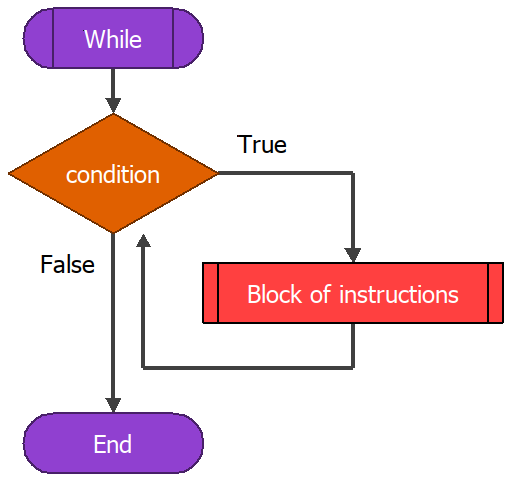
\includegraphics[scale=.24]{img/While_Chart.png}
\caption{while flowchart}
    \end{figure}
\end{frame}
\begin{frame}[fragile]{Loops}
    \tit{While loop with else}
    \texttt{while} loop can have an optional \text{else}. The \text{else} body is executed if the condition is \texttt{False} 
\begin{lstlisting}[numbers=left,showstringspaces=false,language=python]
counter = 0
while counter < 3:
    print("Inside while body")
    counter = counter + 1
else:
    print("Inside else body")
\end{lstlisting}        
\end{frame}
\begin{frame}[fragile]{Loops}
    \tit{\texttt{for} loops}
    \begin{itemize}
        \item The \texttt{for} loop allows to execute a block of instructions multiple times. In fact, this loop is used to iterate over iterable objects.
        \item An {\bf iterable objects} is a sequence of items capable of returning its members one by one, for example \texttt{list} and \texttt{strings} are iterable objects.
    \end{itemize}
    The \texttt{for} loop  syntax in python is:
\begin{lstlisting}[showstringspaces=false,language=python]
for loop_var in iterable_object:
    for_block #body
\end{lstlisting}   
The variable \texttt{loop\_var} take the values of the items of the iterable object. Loop continues until the variable reach the last item in the sequence.


The body of the loop must be indented.
% TODO: range() function
\end{frame}
\begin{frame}[fragile]{Loops}
    \exercise{Draw the flowchart of for loop}
% \begin{figure}
%         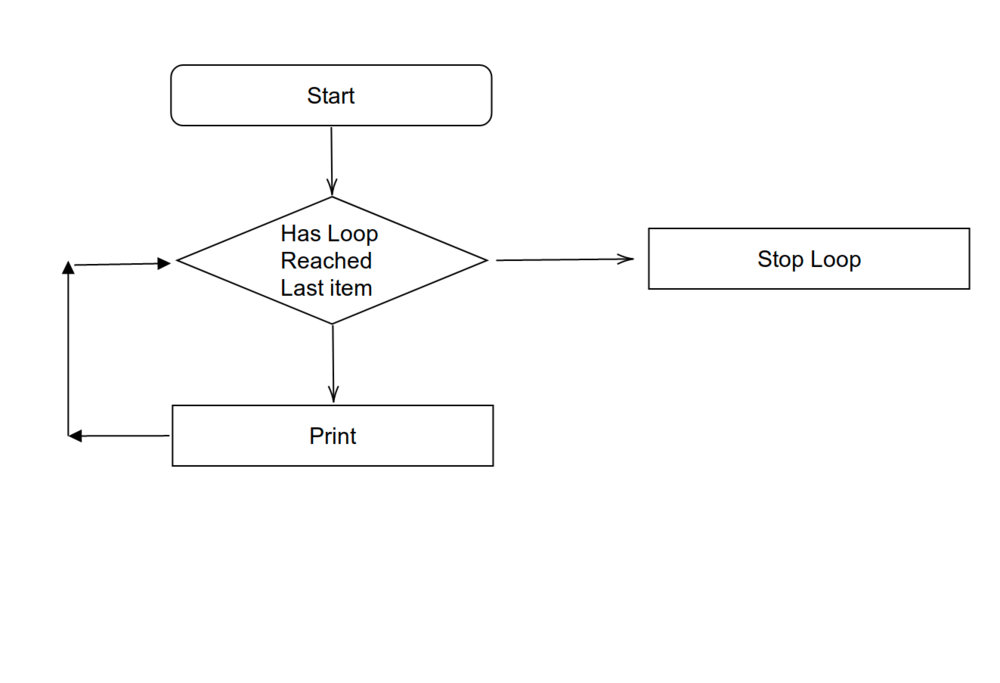
\includegraphics[scale=.24]{img/For_Chart.png}
% \caption{for flowchart}
%     \end{figure}
\tit{Example: Python \texttt{for} Loop}
\begin{lstlisting}[numbers=left,showstringspaces=false,language=python]
word="NHSM"
for letter in word:
    print(letter)
\end{lstlisting}        
\end{frame}
\begin{frame}[fragile]{Loops}
    \tit{\texttt{range()} function}
    In python, we can use the {range()} function to generate a sequence of numbers.
    \pause
    The usage of range function is as follows:
        $$\texttt{range([start], stop,[step\_size])}$$
\begin{align*}
    \texttt{start}: &\text{(Optional). An integer number specifying at which position to start.}\\ 
                    &\text{Default is 0.}\\
    \texttt{stop}:&\text{An integer number specifying at which position to stop}\\
                  & \text{(not included).}\\
    \texttt{step}:&\text{(Optional). An integer number specifying the incrementation.}\\
                  &\text{Default is 0.}
\end{align*}
\pause
    Try this
    \begin{lstlisting}[numbers=left,showstringspaces=false,language=python]
print(range(10))
print(list(range(10)))
print(list(range(2, 8)))
print(list(range(2, 20, 3)))
    \end{lstlisting}        
\end{frame}
\begin{frame}[fragile]{Loops}
    \tit{Examples}
    \begin{lstlisting}[numbers=left,showstringspaces=false,language=python]
        #example1
        for i in range(9):
            print(i)
        else:
            print("No items left.")
        #example2 (else)
        digits=[6,2,9]
        for digit in digits:
            print(digit)
        else:
            print("No items left.")
        #example3
        # Program to iterate through a list using indexing
        names = ['Omar', 'Mohamed', 'Ali']
        # iterate over the list using index
        for i in range(len(names)):
            print("His name is", names[i])
    \end{lstlisting}
\end{frame}
\begin{frame}[fragile]{Loops}
    \tit{Loops}
    \exercise{Write a program which print the following messages\\
    "Hi Student 1"\\
    "Hi Student 2"
    

    \hspace{1cm} \vdots\\
    "Hi Student 90"\\
    "Hi Student 100"}
   \pause

    Will you print all the messages using 100 \texttt{print} function?!! So What we can do ?
\pause    
    \begin{block}{}
        In programming, loops are the statements that allow executing the same block of instructions multiple times.


        Python has essentially two types of loops: \texttt{while loops} and \texttt{for loops}.
    \end{block}
\end{frame}
% \begin{frame}[fragile]{Loops}
%     \tit{}
%     \begin{lstlisting}[numbers=left,showstringspaces=false,language=python]
%     \end{lstlisting}        
% \end{frame}
% \begin{frame}[fragile]{Loops}
%     \tit{}
%     \begin{lstlisting}[numbers=left,showstringspaces=false,language=python]
%     \end{lstlisting}        
% \end{frame}
% \begin{frame}[fragile]{Loops}
%     \tit{}
%     \begin{lstlisting}[numbers=left,showstringspaces=false,language=python]
%     \end{lstlisting}        
% \end{frame}
% \begin{frame}[fragile]{Loops}
%     \tit{}
%     \begin{lstlisting}[numbers=left,showstringspaces=false,language=python]
%     \end{lstlisting}        
% \end{frame}
% \begin{frame}[fragile]{Loops}
%     \tit{}
%     \begin{lstlisting}[numbers=left,showstringspaces=false,language=python]
%     \end{lstlisting}        
% \end{frame}
% \begin{frame}[fragile]{Loops}
%     \tit{}
%     \begin{lstlisting}[numbers=left,showstringspaces=false,language=python]
%     \end{lstlisting}        
% \end{frame}